%This kind of comments need to go to the dicussion. As mentioned above here you report on the results. So the numbers, tables and images. You can write the the rod X was better vissible than Y. One iquid waseasier to fill than other. But what you thing is more useful and why (considering all pros and cons) you need to put in the dicussion. That is why it is called discussion :)



\chapter{Discussion}
% o Interpretation of results, putting them in context with literature
% o Discuss only results which were presented in the results section and do not repeat them one by one
% o Which impacts have your results on the scientific community?
% o provide an assessment of the weaknesses and strengths of your work
% o At least 5 pages

\section{Phantom design}

To be able to assess the spacial distortion of an MRI scan, a rigid object with known dimensions needs to be scanned so the cross referencing to the ground truth can be performed.
Such phantoms are commercially available, but often expensive and designed for a specific calibration protocol.
Some institutions build their own to fulfil exactly the requirements of a given application.
The scanner used at the AKH is a relatively rare model, which is why no off-the-shelf phantom that would fit its coil is available.

A previously used phantom did not fill the whole FOV, while at the same time weighing about 45kg.
This was due to the fact that it resembled a cuboid water tank with a thin filled or solid plastic rod construction inside.
As the peripheral zones of the FOV are those where distortion is most pronounced, a bigger phantom was needed to assess those regions.
The new design deals reaches the outer regions and weighs much less at the same time.\\

Due to the underlying physics, plastics are not visible in MR scans, but CT scans visualize them. 
See figure \ref{fig:sagittal_comparison} for a comparison (MRI/CT visibility).
Therefore, it was decided to use plastic rods with a suitable fluid filling.
Such a liquid should be easily produced, non-toxic and yielding sufficient signal in MRI scans.

Commercially available phantoms often resemble water tanks containing rigid plastic grids used as reference.
While this design results in stronger signal, its weight might be considered as inconvenient.
There are few brands offering solutions utilising liquid fiducial markers in the shape of pellets.
They are arranged in a regular pattern surrounded by air or plastic.
The AKH's design, however, relies on replaceable rods, which makes it a novelty.

\subsection{Observed issues}

Interestingly, all water based solutions seemed to have evaporated partly.
As the rod filled with liquid \textbf{\#15} has dried starting at the end with the plastic stopper, it seems likely that, at least in this particular case, the plastic stopper did not effectively close the rod.
It might also be that the rod itself does not prevent volatile liquids from escaping slowly.
This was tested in a small experiment where a filled rod with only both its ends submerged in water, but the middle part in contact with air was observed over a period of some months (upright rod placed in a glass of water so that the lower end was surrounded by water, a plastic cup of water with a hole in its bottom through which the rod was stuck, glued to seal the hole).
Just like in all other rods which were not partly submerged in water, air bubbles formed along its wall.
This indicates that not (only) the plastic stopper, but the wall (which was the only part of the rod that was in contact with air) is too thin to keep the filling from evaporating.
An airtight container might have led to other conclusions regarding the formation of air bubbles.
It is hard to tell if they were caused by evaporation only or if dissolved gases played a role, too.
Whatever the reasons are, the use of water based liquids seems to be suboptimal.
Despite this, the observed behaviour will still be discussed as different phantom design might benefit from drawn conclusions.

\section{Tested solutions}

For measuring the position of the rods in the CT scans, the plastic rods without filling would be enough already.
That is why the visibility of the liquids on CT is not important at all.
Hollow plastic rods would not be visible on the MRI scans, though.
From now on 'signal (strength)' or 'visibility' will refer to MRI scans only (see table \ref{tab:visibility}).

\subsection{Thoughts about choosing possible candidates}

The tested solutions were chosen for a number of reasons:
\begin{itemize}
\item Generally, imaging techniques aims for a high signal-to-noise ratio. Therefore, liquids resulting in brighter pixels are favoured.
\item The amount of gas in the rods should be minimised.
\item If air bubbles form, tilting the entire phantom slightly should be enough to move them to one side. The FOV of the MRI scanner is too small to show the entire phantom anyway.
\item Most tested fluids are based on water, as they are easily removed from the rods leaving little residue.
Therefore, filling the rods again with a different liquid would be possible if ever needed.
\item Preferably, the components which are chosen to be used for the entire phantom should be non-toxic.
\end{itemize}

\vspace{1cm}

Rod \textbf{\#1} was filled with plain distilled water and intended to be used only as a reference.
It was clear from the beginning that it would not result in high signal and was never considered a possible filling.

\subsubsection{Aiming for high SNR}
To achieve a better SNR, liquids \textbf{\#2} to \textbf{\#10} and \textbf{\#14} to \textbf{\#15} are based on a solution of sodium chloride ($NaCl$ concentration of $0.36 \, g/L$) and copper(II) sulfate pentahydrate ($CuSO_4\cdot5H_2O$ concentration of $1.96 \, g/L$ as suggested by AAPM MR Subcommittee \cite{Jackson2009};  \textbf{\#3} and \textbf{\#4} contain double and ten-fold the concentration) in distilled water.
Most of these liquids resulted in an about 5 times brighter signal than plain distilled water.
Regarding the toxicity of $CuSO_4\cdot5H_2O$, the minimum dose to have caused acute toxic effects in humans is reported to be $11 mg/Kg$.
%As the concentration of $CuSO_4\cdot5H_2O$ is only $1.96 \, g/L$, even a young patient of 4 years and $15kg$ would need to drink more than 80mL to reach that threshold.
%Also, ingestion usually leads to vomiting triggered by its irritating effect on the gastrointestinal tract, which would stop further (more severe) toxic effects from happening.
%Keeping the scanner bed clean and checking the phantom for leakage before and after use should be sufficient to prevent an intoxication.
% http://pmep.cce.cornell.edu/profiles/extoxnet/carbaryl-dicrotophos/copper-sulfate-ext.html

\vspace{1cm}

Primovist (\textbf{\#11} to \textbf{\#13}) is a common contrast agent used for MRI scans \cite{VanBeers2012, Rohrer, primovist} intended to yield an even stronger signal than $CuSO_4\cdot5H_2O$ based liquids.
The major drawback is its tendency to separate from the water and stick to the container's wall.
This results in low signal at the centre and high signal along the wall, which would not necessarily pose a problem, but as the liquid forms bubbles, it is not guaranteed that the walls would be covered homogeneously.
The uneven distribution might result in wrong calculations, especially if the software tool is not programmed to cope with this behaviour.
At the same time the removal of such a solution would be hardly possible.

\subsubsection{Handling dissolved gas}
Unfortunately, dissolved gases may eventually leave the liquid and form air bubbles trapped in the rod.
To improve the mobility of trapped air bubbles, generic washing-up soap was added (\textbf{\#5}, \textbf{\#6}, and \textbf{\#7}; suggestion by Data Spectrum Corporation \cite{bubbles}).
%The smallest amount of 1 g/L was already enough to result in sufficient mobility and an even lower concentration might also be acceptable.
The higher concentrations of soap were tested as reference.
%Interestingly, the rod filled with this solution contained the least amount of gas after 2 months.
If the liquid should happen to leak from the rod, the relatively low concentration of soap would not add to its toxicity.
%The visibility recorded was among the higher candidates, too.
For those reasons, and because the liquid is cheap and easy to produce, it appears to be a promising candidate.

\vspace{1cm}

Liquids \textbf{\#8} ($0.36 g/L$), \textbf{\#9} ($3.6 g/L$) and \textbf{\#10} ($36 g/L$) contain ascorbic acid.
Adding this was supposed to reduce forming of air bubbles by binding dissolved oxygen and eventually degrade to dehydro-ascorbic acid and water.
The amount suggested by \cite{Abtahi2008, Bodannes1979} is $0.00204 \; mol/L$ which corresponds to approx. ($0.36 g/L$).

\vspace{1cm}

In an attempt to limit the forming of gas, \textit{agar} was used in solutions \textbf{\#14} and \textbf{\#15}.
Agar and agarose are commonly used as basic reference material for MRI phantoms \cite{Bucciolini1989, Mathur-DeVre1985}
%Since the produced gel cannot be removed from the rods as easily as liquid candidates, and forming air bubbles were also not moving, agar is not suited for this phantom.

\subsubsection{Non water-based liquids}
As an alternative to water based solutions, two oils were proposed.
Since oil is neither soluble in air, nor able to evaporate, a rod completely filled with oil should stay free from air bubbles.
Yet, oil is not as easily removed from a rod as a water based liquid.
At the same time, it might not be necessary to ever replace the oil.
Once filled, the rods could be used until the surrounding plastic breaks or starts leaking.
Using vegetable oil would be a non-toxic solution, but has been ruled out as a filling from the beginning, because it would eventually rot.
Synthetic oil on the other hand does not rot, however, it might be toxic if consumed.
%As the generic motor (\textbf{\#16}) oil resulted in the highest signal intensity of all candidates it seems to be a good alternative to water based liquids.
%The silicon oil (\textbf{\#17}) on, the other side, had a low signal compared to most candidates and is therefore not suited.


\subsection{Choosing a promising candidate}
As all rods containing water continued to lose liquid due to evaporation, only the early forming of air bubbles might indicate whether solutions effectively hinder dissolved gases to result in trapped air bubbles.
Apart from the solutions containing ascorbic acid (\textbf{\#8} ($0.36 g/L$), \textbf{\#9} ($3.6 g/L$)) all water based liquids produced some air bubbles after at least two days (see table \ref{sec:sol-mech}).
Considering the low visibility of \textbf{\#9}, the only suitable water based liquid capable of staying free from air bubbles might be \textbf{\#8}.
At the same time, long-term observations performed in an airtight container might have shown that even \textbf{\#8} only delays the process.
In the case of the used rods, such a conclusion cannot be drawn with certainty.

The rod containing the highest concentration of ascorbic acid showed a yellow colouring, caused by dehydroascorbic acid which is the result of a oxygenation process.
However, as the high concentration in \textbf{\#9} and \textbf{\#10} led to a radical reduction in signal with the tested MRI sequence, this solutions is not considered a suitable filling anyway.

Primovist (\textbf{\#11} to \textbf{\#13}) lead to a good signal, but its limited mobility of air bubbles; its tendency to accumulate along the wall rule it out as a candidate.

If the forming of  a small amount of gas is not considered a problem, adding soap appears to be a reasonable solution.
The smallest tested amount of soap (\textbf{\#5}, 1 g/L) was already enough to result in sufficient mobility of air bubbles, and an even lower concentration might also be acceptable.
Interestingly, the rod filled with this solution contained the least amount of gas after 2 months, but this might be because the particular rod closed better than the others.
The visibility recorded was among the higher candidates, too.
For those reasons, and because the liquid is cheap and easy to produce, it is a promising candidate.

Solutions containing \textit{agar} (\textbf{\#14} and \textbf{\#15}) are even harder to remove from rods if not impossible.
As they might lead to air bubbles, too, which cannot be moved to either side of the rod, agar is not suited for this phantom.

Finally, the synthetic motor oil (\textbf{\#16}) resulted in the highest signal intensity of all candidates.
Besides the question of its toxicity, it seems to be a good alternative to water based liquids.
The silicon oil (\textbf{\#17}) on, the other side, had a low signal compared to most candidates and is therefore not suited. \\

The question of which liquid to use as a filling is adressed in section \ref{sec:filling}.


\section{Distortion}

\subsection{Calculation Methods}
\texttt{DC} and warp calculated with the simple and iteration method do not differ much.
Moreover, both methods choose very similar thresholds for their calculations (see header of appended '.txt' output file)
As the simple method uses additional information on the rod's true dimension, it is supposed to yield accurate, reliable results.
The iteration process, oblivious to the imaging modality, supports this claim as it produces very similar numbers.\\

The biggest difference in the results obtained with both methods are the values in the region of the air bubble in rod \#5:
Slices 303-310 in table \ref{tab:spit-out-5} mark the area where the maximum brightness dropped significantly due to the absence of liquid (see figure \ref{fig:ph2_MR_x100_brightness}).
The simple method for finding the COM did not manage to calculate coordinates in this region, due to the lack of pixels above the threshold based on the reference slice (which was ~827; see appendix).
Consequently, warp and DC for MRI were set to '-1'.
However, the iteration method tried various thresholds and settled for the one resulting in the highest average DC for the whole scan.
As slices with values of '-1' influence the average dramatically, the chosen threshold is low enough (~339; see appendix) to include some of the brightest pixels in slices 303-310.

\begin{figure}[!tbh]
\centering
	\begin{subfigure}[b]{0.32\textwidth}
		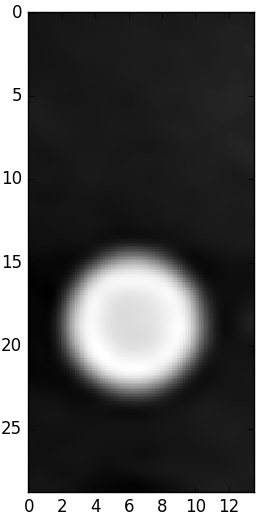
\includegraphics[width=\linewidth]{../fig/python/ph2/brightness/ph2_CT_pane@175}
		\caption{slice 175}
		\label{fig:ph2_CT_x100_pane_0}
	\end{subfigure}
	\begin{subfigure}[b]{0.32\textwidth}
	  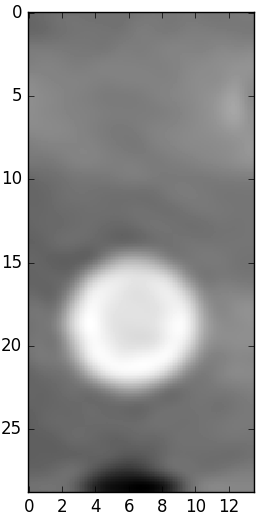
\includegraphics[width=\linewidth]{../fig/python/ph2/brightness/ph2_CT_pane@176}
	  \caption{slice 176}
	  \label{fig:ph2_CT_x100_pane_1}
	\end{subfigure}
	\begin{subfigure}[b]{0.32\textwidth}
	  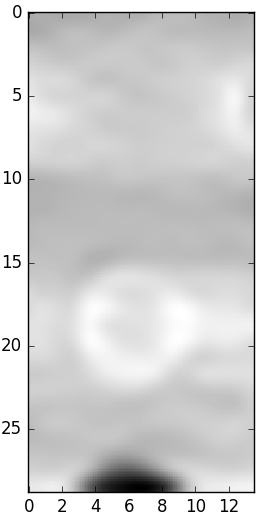
\includegraphics[width=\linewidth]{../fig/python/ph2/brightness/ph2_CT_pane@177}
	  \caption{slice 177}
	  \label{fig:ph2_CT_x100_pane_2}
	\end{subfigure}
  \caption{Slices at edge of plastic pane in CT image showing rod \#5 (true colours): a black crescent remains at the bottom where there is a hole in the pane that is not filled with a rod at the moment}
  \label{fig:ph2_CT_x100_pane}
\end{figure}

\subsection{Irregularities}
All obtained CT scans include a region where the plastic panes are visible.
Figure \ref{fig:ph2_CT_x100_pane} shows how the plastic pane makes it impossible to define the rod on the CT image.
These areas cannot be used for distortion assessment as the COM cannot be calculated reliably.
Figures \ref{fig:ph2_CT_x100_brightness} and \ref{fig:ph3_CT_x100_brightness} exhibit spikes in the average brightness where the image shows a plastic pane.
The script recognised this difference and marked all affected slices as 'irregular'.
Consequently, in table \ref{tab:spit-out-5} and \ref{tab:spit-out-16}, the values of the COM shift ($warp_x$, $warp_y$, $warpM$); the DC for CT using the CT-centroid ($DC_{CT}$); and the DC for MRI using the CT-centroid ($DC_{MR(CT-COM)}$) are all set to '-1'.

In the future, the threshold value used to determine a significant change in brightness could be automatically chosen based on the image modality and the image size.

\subsection{Measured distortion - Rod \#5}

Figure \ref{fig:MR_x100_centroids} visualises the centroid shift at interesting slices of rod \#5.
It is clearly visible that the shift is bigger at the end of the rod (slice 0) compared to a slice close to its middle (slice 171).
The values of $warpM^*$ in table \ref{tab:spit-out-5} verify this (1.0623mm > 0.6926mm).
Furthermore, the distortion measured at the location of the air bubble (slice 304) shows a maximum for the COM shift ($warpM^*$ = 1.5748mm) and a minimum for the DC ($DC^*_{MR}$ = 0.6762).
These values originate not from true spatial distortion, but are caused by the presence of gas in the rod.
Since the bubble floated on top of the liquid, the COM shift is most pronounced in the y direction (up-down) as shown by figure \ref{fig:ph2_warpXY_x100}.
The overall impact on the area of 110mm to 140mm is clearly visible in figures \ref{fig:ph2_warpMagnitude_x100} and \ref{fig:ph2_DC_x100}.
In conclusion, it is imperative for the distortion assessment to exclude bubbles from the FOV.

\subsection{Measured distortion - Rod \#16}

Similar to the findings for rod \#5, the distortion is bigger in the peripheral regions of the FOV (see figure \ref{fig:ph3_DC_x100}).
Interestingly, the y shift changes its orientation around the centre (see figure \ref{fig:ph3_warpXY_x100}).
This might be a local feature of the distortion and cannot be put in relation, because no distortion map of the entire FOV is available yet.

As rod \#16 does not contain any air bubbles, the brightness plotted in figure \ref{fig:ph3_MR_x100_brightness} shows no sudden drops.
However, the left hand side has a drastically lower signal strength than the right.
A closer look revealed that rod \#16 contained oil of two different colours.
It seems that some residue of the other oil, which was injected into rod \#17, was still present in the syringe when rod \#16 was filled.
To avoid this, the injecting syringe and the capillary were flushed with the next liquid before injection.
This procedure was not enough to clean it thoroughly.
The liquids separated into parts with different density while the rod was stored upright and were still distributed unevenly during imaging.
To avoid this problem in the future, a new and unused syringe should be used for filling.\\

It is likely, that this influenced the calculated warp and DC as the lighter oil (which results in a different signal strength) floated on top of the other, resulting in an unwanted shift of the calculated COM.
This might explain why the y shift changes its orientation close to the isocentre as this is the point where the signal intensity starts to change, too.
To be sure of the actual impact of the oil mix on the distortion assessment, a new rod should be filled and the imaging repeated.
For now, the already gained results will be used as no new measurement could be obtained in the limited time that the scanner is available for such experiments.


In the region beyond -330, there is a drop of the DC for the CT.
Investigations revealed that this is caused by adhesive tape attached to the rod to hold it in place during transport from the CT scanner to the MRI scanner.
The values calculated for this area are most likely influenced by this.


\subsection{Effect of resampling}


Figures \ref{fig:ph2_warpMagnitude_x1-100} and \ref{fig:ph3_v2_warpMagnitude_x1-100} depict the measured $warpM^*$ of rod \#5 and \#16 for x1 and x100 resample rates.
The location shift calculated with x1 and x100 resample rate are relatively close (see tables \ref{tab:Delta-resample_5} and \ref{tab:Delta-resample_16}).\\

The calculated DCs for the scans in original CT resolution (x1) are shown in figures \ref{fig:ph2_DC_x1} and \ref{fig:ph3_DC_x1} and for a x4 finer resolution in figures \ref{fig:ph2_DC_x4} and \ref{fig:ph3_DC_x4}.
Compared to the DCs of the x100 resampled scans (figures \ref{fig:ph2_DC_x100} and \ref{fig:ph3_DC_x100}), the low resolution x1 yields significantly less smooth curves.
A resample rate of x4, on the other hand, is already much closer to the quality of the x100 scans.\\

While the original resolution might be sufficient for the calculation of the COM shift, the DC calculation benefits a lot from a interpolated image.
It is easier to spot significant changes as the plot shows less jumps.
At the same time, the computing time for calculations scales with the resolution of the images and should be kept minimal, because a future assessment would include more than 300 individual rods.

Now that the appearance of the curves has been addressed, it will be discussed how the calculated distortion varies with increased resample rate.

\subsubsection{Rod \#5}

Table \ref{tab:Delta-resample_5} lists the expectancy and standard deviation ($\sigma_\Delta$) of the difference between the calculated distortion for x1 and x100 resample rate of rod \#5:

The expectancy value $E$ was calculated as the sum of the difference in each slice over the number of slices; it is the average difference.
A random deviation should result in some slices with positive and some with negative local differences.
Therefore, the average should be close to zero.
Otherwise, an increased resample rate would either result in an overall drop or rise of measured distortion.
Indeed, $E$ is relatively small compared to the typical COM shift (even smaller than $\sigma_\Delta$), which indicates that the increased resample rate does only result in a smoother curve, but not in very different values overall.

The COM shift mostly lies in a range of 0.5 to 0.7mm; $\sigma_\Delta$ is approximately one order of magnitude smaller.
To verify whether this hints at increased accuracy or not, an external reference would be needed.
In any case, a difference of less than $0.1mm$ would not influence treatment planning and can be regarded negligible.

The value of the MRI DC lies between 0.9 and 1 (except for the air bubble region); $\sigma_\Delta$ is roughly a 45th of the average DC value ($0.9/0,02$). This is small enough to be neglected, too.

\begin{table}[!tbh]
 \centering
\begin{tabular}{l|rr}
                    & E         & $\sigma_\Delta$   \\ \hline
$\Delta warpM^*$ [mm]  & 0.038     & 0.058    \\
%$\Delta DC^*_{CT}$         & 0.002245  & 0.006838 \\
$\Delta DC^*_{MRI}$         & 0.000518  & 0.019070 \\
$\Delta DC^*_{MRI(CT-COM)}$ & -0.008905 & 0.022050
\end{tabular}
\caption{Expectancy and standard deviation of difference between calculated distortion for x1 and x100 resample rate; rod \#5}
\label{tab:Delta-resample_5}
\end{table}

\begin{figure}[!tbh]
    \centering
    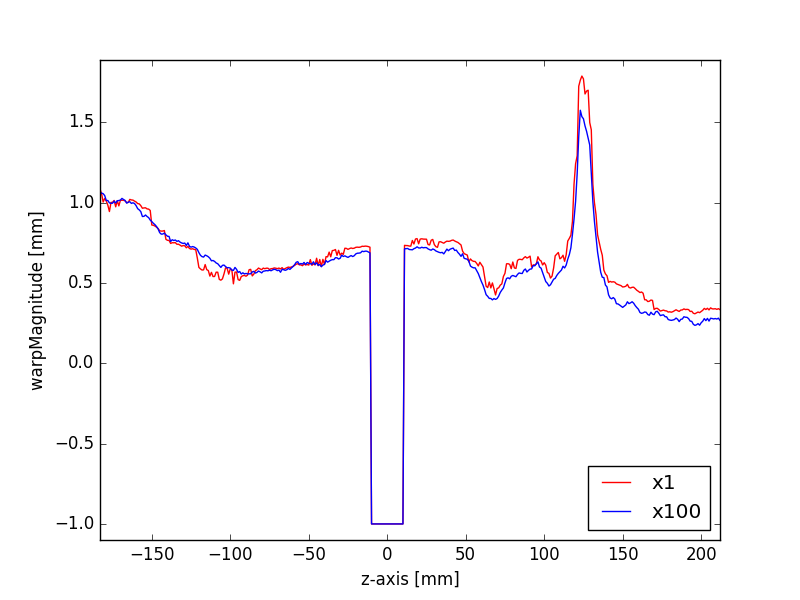
\includegraphics[scale=0.6]{../fig/python/ph2/warp/warpMagnitude_x1-100_iter.png}
    \caption{Rod \#5: warp Magnitude [$mm$] (iteration method), CT-MRI x1 and x100; plastic pane from $-10mm$ to $10mm$, bubble at about $110mm$ to $135mm$}
    \label{fig:ph2_warpMagnitude_x1-100}
\end{figure}

\begin{figure}[!bth]
    \centering
    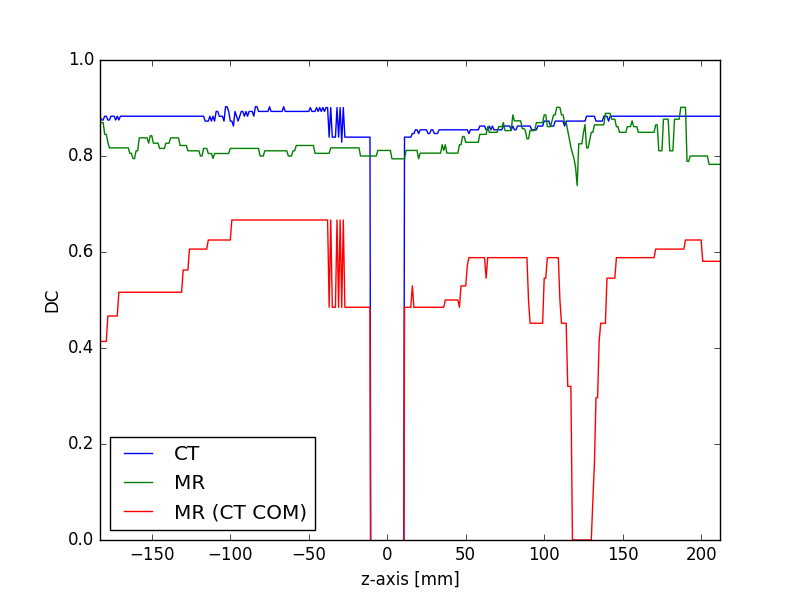
\includegraphics[scale=0.6]{../fig/python/ph2/dice/ph2_DC_x1_iter.png}
    \caption{Rod \#5; x1: DC (iteration method) for CT \& MRI \& MRI (using CT COM); plastic pane from $-10mm$ to $10mm$, bubble at about $110mm$ to $135mm$}
    \label{fig:ph2_DC_x1}
\end{figure}

\begin{figure}[!bth]
    \centering
    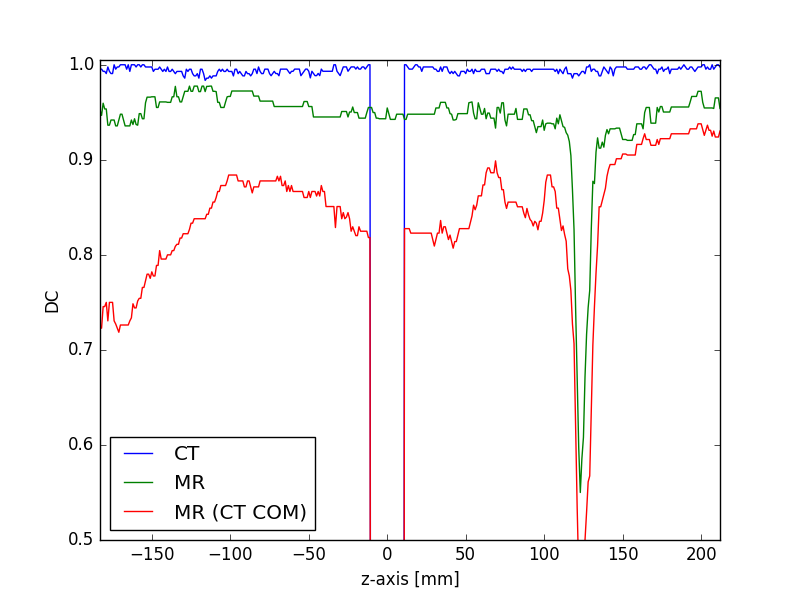
\includegraphics[scale=0.6]{../fig/python/ph2/dice/ph2_DC_x4_iter.png}
    \caption{Rod \#5; x4: DC (iteration method) for CT \& MRI \& MRI (using CT COM); plastic pane from $-10mm$ to $10mm$, bubble at about $110mm$ to $135mm$}
    \label{fig:ph2_DC_x4}
\end{figure}

\clearpage

\subsubsection{Rod \#16}

Table \ref{tab:Delta-resample_16} lists the expectancy and standard deviation $\sigma_\Delta$ of the difference between calculated distortion for x1 and x100 resample rate of rod \#16:

Again, the expectancy $E$ is relatively small; hinting at a low overall shift of the calculated values.

Just like with rod \#5, $\sigma_\Delta$ for the COM shift is approximately one order of magnitude smaller than the occurring warp and can therefore also be regarded a negligible.

Similarly, $\sigma_\Delta$ for the MRI DC is approximately a 45th of the average DC value ($0.9/0,02$) and can be neglected.

\begin{table}[!tbh]
\centering
\begin{tabular}{l|rr}
                    & E         & $\sigma_\Delta$   \\ \hline
$\Delta warpM^*$ [mm]  & 0.005     & 0.025    \\
%$\Delta DC^*_{CT}$         & -0.001849  & 0.007117 \\
$\Delta DC^*_{MRI}$         & 0.004835   & 0.019823  \\
$\Delta DC^*_{MRI(CT-COM)}$ & 0.012554   & 0.019429
\end{tabular}
\caption{Expectancy and standard deviation of difference between calculated distortion for x1 and x100 resample rate; rod \#16}
\label{tab:Delta-resample_16}
\end{table}

\begin{figure}[!tbh]
    \centering
    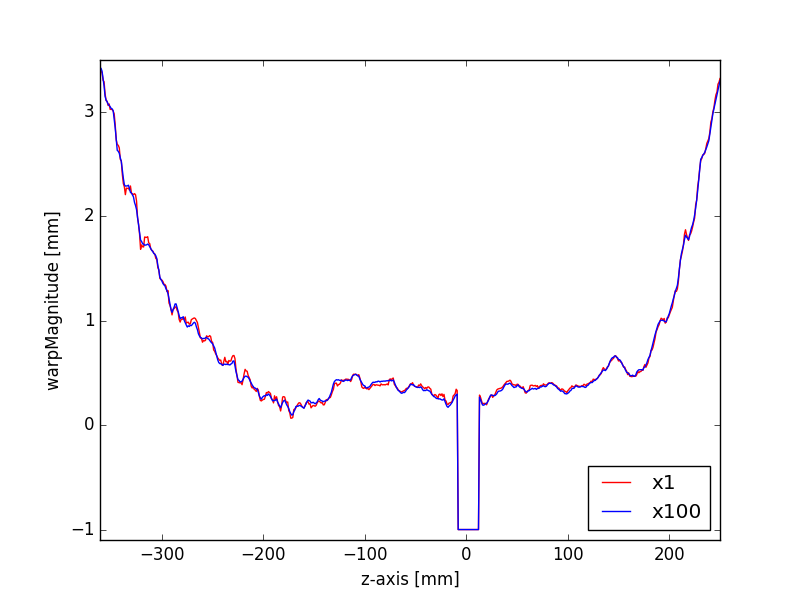
\includegraphics[scale=0.6]{../fig/python/ph3_v2/warp/ph3_MR_v2_x1-100_warpMagnitude_iter.png}
    \caption{Rod \#16: warp Magnitude [$mm$] (iteration method), CT-MRI x1 and x100; plastic pane from $-8mm$ to $12mm$}
    \label{fig:ph3_v2_warpMagnitude_x1-100}
\end{figure}

\begin{figure}[!tbh]
    \centering
    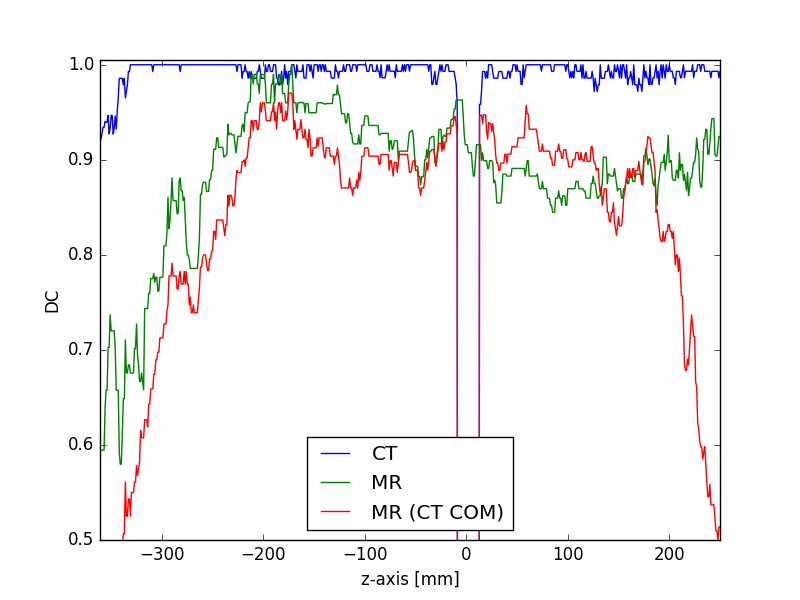
\includegraphics[scale=0.6]{../fig/python/ph3_v2/dice/ph3_MR_v2_x1_DC_iter.png}
    \caption{Rod \#16; x1: DC (iteration method) for CT \& MRI \& MRI (using CT COM); plastic pane from $-8mm$ to $12mm$}
    \label{fig:ph3_DC_x1}
\end{figure}

\begin{figure}[!tbh]
    \centering
    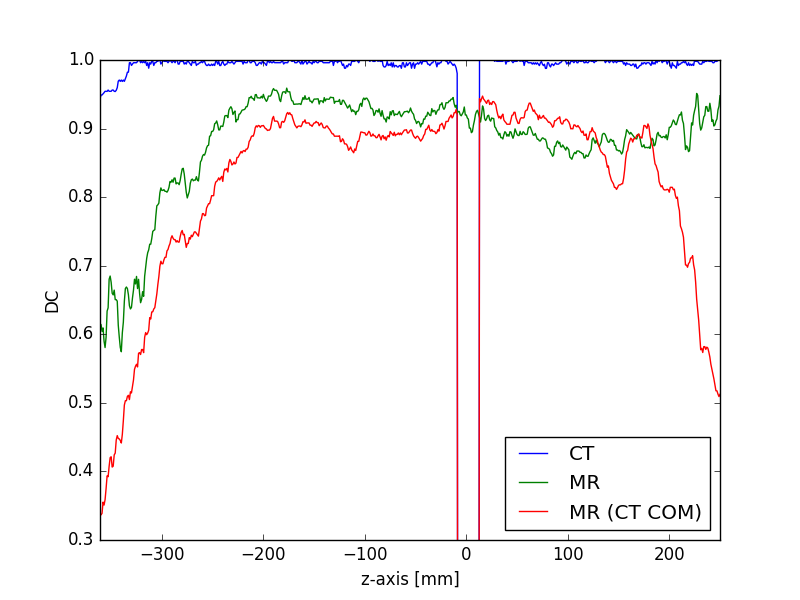
\includegraphics[scale=0.6]{../fig/python/ph3_v2/dice/ph3_MR_v2_x4_DC_iter.png}
    \caption{Rod \#16; x4: DC (iteration method) for CT \& MRI \& MRI (using CT COM); plastic pane from $-8mm$ to $12mm$}
    \label{fig:ph3_DC_x4}
\end{figure}